% Systematic literature review: Reinforcement learning for investigating, acting and escalating
% in IT incident triage and response.
%
% Build from this folder:   ..\..\tools\tectonic.exe Opol_Charis_Systematic_Literature_Review.tex
% Before building after a change to the data, regenerate tables and references:
%                           python -I audit/generate.py
% See README.md for the project layout.

\documentclass[journal]{IEEEtran}

\usepackage{fontspec}
\setmainfont{texgyretermes}[Extension=.otf,UprightFont=*-regular,BoldFont=*-bold,ItalicFont=*-italic,BoldItalicFont=*-bolditalic]
\usepackage{amssymb}
\usepackage{booktabs}
\usepackage{tabularx}
\usepackage{longtable}
\usepackage{array}
\usepackage{graphicx}
\usepackage{xcolor}
\usepackage{tikz}
\usetikzlibrary{positioning,arrows.meta,fit,calc}
\usepackage{pgfplots}
\pgfplotsset{compat=1.17}
\usepackage{cite}
\usepackage[hyphens]{url}
\usepackage[colorlinks=true,linkcolor=black,citecolor=black,urlcolor=blue]{hyperref}

\newcolumntype{L}{>{\raggedright\arraybackslash}X}
\newcolumntype{P}[1]{>{\raggedright\arraybackslash}p{#1}}
\newcommand{\todo}[1]{\textcolor{red}{[TO DO: #1]}}
\newcommand{\orcid}{\href{https://orcid.org/0009-0003-7417-7984}{\raisebox{-0.15em}{
\includegraphics[height=0.95em]{figures/orcid.png}}}}
% Table row files are read with the primitive \input so they can sit inside tabular environments.
\makeatletter
\newcommand{\inputrows}[1]{\@@input #1 }
\makeatother

% Abstract and keyword headings with a colon instead of the class's em dash.
\renewenvironment{abstract}{\par\noindent\small\bfseries\textit{Abstract:}\ }{\par\vspace{0.6\baselineskip}}
\renewenvironment{IEEEkeywords}{\par\noindent\small\bfseries\textit{Index Terms:}\ }{\par\vspace{0.6\baselineskip}}

% Generated by audit/generate.py from review_data.py and the screening record.
\newcommand{\NScopus}{3394}
\newcommand{\NACM}{1000}
\newcommand{\NIEEE}{5}
\newcommand{\NIdentified}{4399}
\newcommand{\NDuplicates}{73}
\newcommand{\NAfterDedup}{4326}
\newcommand{\NAutoType}{1462}
\newcommand{\NAutoYear}{32}
\newcommand{\NAutoA}{2270}
\newcommand{\NAutoB}{431}
\newcommand{\NAutoString}{2701}
\newcommand{\NAuto}{4195}
\newcommand{\NScreened}{131}
\newcommand{\NExclTA}{84}
\newcommand{\NSought}{47}
\newcommand{\NNotRetrieved}{7}
\newcommand{\NNotRetClosed}{6}
\newcommand{\NNotRetNoRecord}{1}
\newcommand{\NAssessed}{40}
\newcommand{\NExclFT}{6}
\newcommand{\NIncluded}{34}
\newcommand{\NPOne}{25}
\newcommand{\NPTwo}{22}
\newcommand{\NInclPOne}{20}
\newcommand{\NInclPTwo}{14}
\newcommand{\NFTDetect}{3}
\newcommand{\NYearRecent}{27}
\newcommand{\NYearTwentySix}{17}
\newcommand{\NYearMin}{2020}
\newcommand{\NSetITOPS}{10}
\newcommand{\NSetSOC}{6}
\newcommand{\NSetNET}{11}
\newcommand{\NSetICS}{5}
\newcommand{\NSetDFIR}{2}
\newcommand{\NInfo}{17}
\newcommand{\NAct}{22}
\newcommand{\NDisp}{5}
\newcommand{\NEsc}{7}
\newcommand{\NInfoAct}{7}
\newcommand{\NAllThree}{1}
\newcommand{\NBelief}{4}
\newcommand{\NShield}{5}
\newcommand{\NMask}{6}
\newcommand{\NCostCon}{4}
\newcommand{\NPenalty}{11}
\newcommand{\NNoCon}{8}
\newcommand{\NBlocked}{3}
\newcommand{\NDQ}{31}
\newcommand{\NEff}{19}
\newcommand{\NEscM}{5}
\newcommand{\NComp}{4}
\newcommand{\NAllMetrics}{1}
\newcommand{\NThreeMetrics}{5}
\newcommand{\NRuleBase}{20}
\newcommand{\NRobust}{15}
\newcommand{\NQOne}{25}
\newcommand{\NQTwo}{19}
\newcommand{\NQThree}{19}
\newcommand{\NQFour}{21}
\newcommand{\NQFive}{11}
\newcommand{\NQSix}{9}
\newcommand{\NQSeven}{19}
\newcommand{\NQEight}{5}
\newcommand{\NQHigh}{9}
\newcommand{\NQLow}{12}
\newcommand{\NEnvBench}{6}
\newcommand{\NEnvSim}{13}
\newcommand{\NEnvEmu}{5}
\newcommand{\NEnvData}{6}
\newcommand{\NEnvOps}{3}
\newcommand{\NEnvTestbed}{1}


\begin{document}

\title{Reinforcement Learning for Investigating, Acting and Escalating in IT Incident Triage and Response: A Systematic Literature Review}

\author{Charis~Opol~\orcid\\
Registration No.\ S24B23/003 $\cdot$ B29654@students.ucu.ac.ug\\
Department of Computing and Technology, Faculty of Engineering, Design and Technology\\
Uganda Christian University}

\maketitle

\begin{abstract}
IT support teams must decide what to do with an incident before they know its cause: investigate further, apply a fix, or pass the incident to someone better placed to resolve it. Reinforcement learning (RL) can treat this as a sequence of decisions, but the published work is spread across IT operations, security operations and safe RL. This review asks how RL and related sequential methods have been applied to IT incident handling, which of the three decisions their agents make, how operational rules are enforced, and how the agents are evaluated.

The review follows the PRISMA 2020 guideline. Searches of Scopus, IEEE Xplore and the ACM Digital Library on 23 October 2026 returned \NIdentified{} records. After the removal of \NDuplicates{} duplicates and \NAuto{} records by automated filtering, \NScreened{} records were screened on title and abstract, \NSought{} reports were sought, \NAssessed{} were assessed in full, and \NIncluded{} studies published between \NYearMin{} and 2026 were included. Their quality was appraised with an eight-item checklist, and the evidence was synthesised narratively around five review questions.

There are four main findings. First, only \NBelief{} studies represent the hidden state of an incident with an explicit belief, and most treat it as fully observed. Second, \NInfo{} studies give the agent an explicit information-gathering action, but only \NEsc{} include escalation to a person, and only one combines gathering, a response action and escalation, with the escalation fixed by design rather than learned. Third, rule enforcement is proposed more often than it is measured: \NShield{} studies use a hard filter or shield, and \NBlocked{} report what happens to a blocked or uncertain decision. Fourth, decision quality is measured in \NDQ{} studies but escalation behaviour in \NEscM{} and constraint compliance in \NComp{}, and robustness to changing conditions is tested in \NRobust{}. The evidence is recent, with \NYearRecent{} studies published in 2025 or 2026, and uneven in quality: \NQLow{} studies meet at most two of the eight checklist items. The review concludes that a single policy which learns to investigate, act or escalate for IT service incidents under explicit rules has not been reported, and it sets out the evaluation that such work should include.
\end{abstract}


\begin{IEEEkeywords}
Reinforcement learning, sequential decision-making, POMDP, IT incident management, incident triage, incident response, alert triage, AIOps, root cause analysis, escalation, safe reinforcement learning, PRISMA.
\end{IEEEkeywords}

\begin{table}[!t]
\centering
\caption{Abbreviations Used in This Review}
\label{tab:abbrev}
\footnotesize
\begin{tabularx}{\columnwidth}{@{}lL@{}}
\toprule
Abbreviation & Meaning \\
\midrule
AIOps & Artificial Intelligence for IT Operations \\
CAGE & Cyber Autonomy Gym for Experimentation \\
CMDP & Constrained Markov Decision Process \\
DQN & Deep Q-Network \\
EC / IC & Exclusion criterion / Inclusion criterion \\
ICS & Industrial Control System \\
LLM & Large Language Model \\
MCC & Matthews Correlation Coefficient \\
MDP & Markov Decision Process \\
MTTR & Mean Time to Recovery or Resolution \\
POMDP & Partially Observable Markov Decision Process \\
PPO & Proximal Policy Optimisation \\
PRISMA & Preferred Reporting Items for Systematic Reviews and Meta-Analyses \\
RCA & Root Cause Analysis \\
RL & Reinforcement Learning \\
SO / SRQ & Specific Objective / Systematic Review Question \\
SOC & Security Operations Centre \\
\bottomrule
\end{tabularx}
\end{table}


% ===========================================================================
\section{Introduction}
% ===========================================================================

\IEEEPARstart{O}{rganisations} depend on IT services that are expected to remain available, and incident management is the process that restores those services when they fail. Chen et al.\ describe it as the process of detecting a service problem, creating an incident, determining its cause, restoring the service, and capturing knowledge to prevent a recurrence~\cite{chen2020}. Triage is the stage at which a reported incident is assessed and directed towards resolution. Chen et al.\ define it as engaging the team responsible for investigating the problem~\cite{chen2020}, and Remil et al.\ use the term more broadly for the prioritisation, assignment and classification of incidents~\cite{remil2024}. In both descriptions, triage is a set of decisions made before the cause of the incident is known.

These decisions are difficult because the evidence available when they are made is often incomplete or conflicting. In their study of incident management at Microsoft, Chen et al.\ found that distinct problems can produce similar symptoms, so that the symptoms alone may not identify the responsible team~\cite{chen2020}. Remil et al.\ note that data in real IT environments is commonly noisy and incomplete~\cite{remil2024}. Yet many triage models produce one prediction per incident report and are evaluated with classification or ranking metrics~\cite{remil2024}. A model of this kind returns an answer for every report. It has no way to state that more evidence is needed first, and no way to pass the incident to a person.

Reinforcement learning (RL) offers a different framing. In RL, an agent learns a policy, which is a rule for choosing actions, by acting in an environment and receiving rewards that reflect the consequences of its actions~\cite{sutton2018}. When the agent cannot observe the true state of the environment, the problem can be described as a partially observable Markov decision process (POMDP), in which the agent keeps a belief about the hidden state and may choose an action for the information it yields, weighing the cost of that information against its value~\cite{kaelbling1998}. Under this framing, triage becomes a sequence of decisions: the agent can gather more evidence, recommend an action, or hand the incident to a human expert.

Two further requirements follow when such an agent is meant for IT operations. The first is that its actions must respect operational rules. A reward signal alone does not ensure this, because penalising an undesirable action in the reward does not guarantee that the agent never selects it~\cite{konighofer2025}, and Remil et al.\ state that automatic healing actions need to be executed safely~\cite{remil2024}. The second is that the agent must know when to involve a person. Learning to defer trains a model to decide when a human should take over~\cite{madras2018}, and recent work treats escalation as a decision with costs in both directions, since a reviewer's attention is limited~\cite{turan2026}.

The literature review for the project of which this review is part (Chapter Two of the project report) found that these strands have developed largely apart. Studies of information gathering let an agent choose between looking further and deciding~\cite{janisch2019,kim2025}, studies of deferral let it choose between deciding and handing over~\cite{madras2018,joshi2023}, and a shielded agent proposed for incident response selects responses without choosing whether to investigate or escalate~\cite{alauthman2026}. That review was thematic and not systematic. It drew on a core set of collected publications and on a database search run on 13 October 2026, which returned 10,694 records that were filtered by keyword and not screened. Its conclusions about gaps were therefore conclusions about the literature it had read. This review replaces that search with a narrower, documented one, screens its results against fixed criteria, and synthesises what the included studies report.

The project plans an RL agent for IT incident triage that chooses among requesting a diagnostic check, recommending a fix that the organisation's operational rules permit, and escalating to a human expert, with every proposal checked by an independent rule-based mechanism. The agent is to be trained and evaluated in simulation. Because this review prepares for that study, it could lean towards the planned design. Three measures limit this. The eligibility criteria were written before screening, the decisions that required interpretation are stated in Section~\ref{sec:screening}, and the outcome of every report sought is listed in Appendix~\ref{app:decisionlog}. These measures do not remove the risk, because the screening and extraction were not independently duplicated (Section~\ref{sec:limitations}).

The review addresses five questions:
\begin{itemize}
\item \textbf{SRQ1:} How have IT incident handling tasks been formulated as MDP, POMDP or RL problems, and how is incomplete or conflicting evidence represented in them?
\item \textbf{SRQ2:} Which decisions do the agents make (gathering information, recommending or taking an action, escalating to a human), and does any study combine all three?
\item \textbf{SRQ3:} How are operational constraints enforced, for example by a shield, action masking, constrained optimisation, a reward penalty or human approval, and what happens when an action is blocked?
\item \textbf{SRQ4:} Which environments, datasets, baselines and evaluation metrics are used?
\item \textbf{SRQ5:} How is robustness to missing, unreliable or ambiguous evidence evaluated, and what results are reported?
\end{itemize}

The general objective is to systematically identify and synthesise peer-reviewed studies that apply RL or sequential decision-making to IT incident management, with attention to how they represent uncertain evidence, which decisions the agent makes, how constraints are enforced, and how the agents are evaluated. Table~\ref{tab:objectives} gives the five specific objectives (SO1--SO5), the question each answers, the research question of the project that it informs, and the gap that motivated it. The gaps in the table are those stated by the project's thematic review before this search; Section~\ref{sec:discussion} returns to each of them in the light of the included evidence.

\begin{table*}[!t]
\centering
\caption{Objectives, Research Questions and Gaps Addressed}
\label{tab:objectives}
\footnotesize
\begin{tabularx}{\textwidth}{@{}P{3.6cm}P{1.1cm}P{2.3cm}L@{}}
\toprule
Specific objective & Review question & Project question informed & Gap that motivated it (from the thematic review) \\
\midrule
SO1: Identify which incident tasks have been formulated as sequential decision problems, and how they represent uncertain evidence & SRQ1 & RQ1 (representation of ambiguous scenarios) & The environments used in the reviewed studies model cyberattacks and microservice faults, and none lets the ambiguity of IT service incidents be varied~\cite{hammar2025,dunsin2025,wang2023hrlhf}. \\
SO2: Classify the decisions the agents make & SRQ2 & RQ2 (investigate, recommend, escalate) & Information gathering and deferral have been studied separately; no reviewed study trained one policy to choose among all three options for IT incident triage~\cite{janisch2019,kim2025,madras2018,joshi2023}. \\
SO3: Analyse how constraints are enforced and what is reported about blocked actions & SRQ3 & RQ3 (rule-based safety mechanism) & Shields have been demonstrated mainly on control tasks, and the reviewed literature did not report how a rule mechanism behaves when the agent can also investigate or escalate~\cite{alshiekh2018,konighofer2025,alauthman2026}. \\
SO4: Catalogue environments, datasets, baselines and metrics & SRQ4 & RQ4 (comparison with baselines) & Decision quality, investigation cost, escalation and constraint compliance had each been measured, but not together for one agent~\cite{remil2024,levy2026,pacella2026}. \\
SO5: Synthesise how robustness to increasing ambiguity is tested & SRQ5 & RQ5 (robustness) & Robustness had been tested for decision accuracy and for the validity of shields, but not for the mix of investigating, recommending and escalating~\cite{kim2025,hammar2025,hamel2026}. \\
\bottomrule
\end{tabularx}
\end{table*}

% ===========================================================================
\section{Methodology (PRISMA Protocol)}
\label{sec:method}
% ===========================================================================

This study is a systematic literature review reported according to the PRISMA 2020 guideline~\cite{page2021} and guided by the review procedure for computing proposed by Kitchenham and Charters~\cite{kitchenham2007}. A systematic approach was chosen because it makes the search, selection and extraction of studies transparent and reproducible, and because the earlier search for the project returned too many records to screen. The design follows the five objectives and questions in Table~\ref{tab:objectives}. The protocol was not registered. Every count reported below is generated from the screening and extraction records that accompany this review (Section~\ref{sec:records}).

\subsection{Information Sources}

Three databases were searched: Scopus, IEEE Xplore and the ACM Digital Library. Scopus was the primary source for its broad indexing. IEEE Xplore was chosen for its coverage of network, service management and security venues, and the ACM Digital Library for software engineering and systems venues, where much AIOps work appears. The searches were run on 23 October 2026. The Scopus and ACM Digital Library searches used the all-fields option of each site. The IEEE Xplore search was limited to open-access records.

Other sources were considered and not used. SpringerLink and SIAM, which were searched for the project's earlier review, were dropped: the SpringerLink export of that search contained no abstracts, and SIAM returned three records. Web of Science was not searched. arXiv was not searched directly, so preprints could have entered only through citation searching, which was planned but not carried out (Section~\ref{sec:other}).

\subsection{Search Strategy}

The search was designed to be narrow. The earlier search had combined a block of terms for the learning approach, a block for uncertainty and oversight, and a block for the incident-management setting. Single words such as ``uncertainty'' and ``triage'' match large bodies of unrelated work, including medical triage and traffic incidents. The new string therefore anchors the review on the intersection of two concepts, the RL or sequential-decision method (block~A) and the IT incident setting (block~B), expressed as exact phrases, and adds a block of decision terms (block~C). Synonyms within a block were joined with OR and the blocks were joined with AND. Table~\ref{tab:keywords} lists the keywords and shows where each appears.

\begin{table}[!t]
\centering
\caption{Keywords and Their Use in the Search Strings}
\label{tab:keywords}
\footnotesize
\begin{tabularx}{\columnwidth}{@{}lLL@{}}
\toprule
No. & Keyword & Block \\
\midrule
1 & Reinforcement learning & A (method) \\
2 & Sequential decision-making & A, as MDP, POMDP and bandit terms \\
3 & POMDP & A \\
4 & IT incident management & B (setting) \\
5 & Incident triage & B \\
6 & Incident response & B \\
7 & AIOps & B \\
8 & Root cause analysis & B, limited to computing systems \\
9 & Escalation & C (decision) \\
10 & Human-in-the-loop & C \\
11 & Information gathering & C \\
12 & Safe reinforcement learning & C \\
13 & Shielding & C \\
14 & Operational constraints & C \\
\bottomrule
\end{tabularx}
\end{table}

Table~\ref{tab:strings} gives the strings exactly as they were run. The Scopus and ACM Digital Library strings are identical. Both end with a fourth group of quoted years; because the searches ran over all fields, these terms match any record that mentions one of the years anywhere and do not restrict the publication year. The IEEE Xplore string differs in four respects: it uses the Scopus proximity operator \texttt{W/5} for the root-cause clause, it spells several terms in full instead of truncating them, it has no year terms, and it was limited to open access. Whether IEEE Xplore interpreted \texttt{W/5} as intended was not tested.

\begin{table*}[!t]
\centering
\caption{Search Strings as Run on 23 October 2026, and Records Exported}
\label{tab:strings}
\footnotesize
\begin{tabularx}{\textwidth}{@{}P{2.4cm}L@{}}
\toprule
Database & String as run \\
\midrule
Scopus (all fields) and ACM Digital Library (all fields) & \texttt{( "reinforcement learning" OR "deep Q-network*" OR "Q-learning" OR "policy gradient" OR "actor-critic" OR "proximal policy optimi*" OR "Markov decision process*" OR "partially observable Markov" OR POMDP OR "contextual bandit*" OR "multi-armed bandit*" ) AND ( "incident management" OR "incident response" OR "incident triage" OR "incident handling" OR "incident resolution" OR "incident mitigation" OR AIOps OR "IT operations" OR "IT service management" OR ITSM OR "site reliability" OR "service desk" OR "help desk" OR "trouble ticket*" OR "ticket routing" OR "ticket assignment" OR "alert triage" OR "alert prioriti*" OR "security operations cent*" OR "automated remediation" OR ( "root cause" AND ( microservice* OR cloud OR "online service*" OR "IT system*" ) ) ) AND ( triage OR escalat* OR defer* OR "human-in-the-loop" OR "human in the loop" OR "human oversight" OR investigat* OR diagnos* OR "information gathering" OR "information acquisition" OR remediat* OR mitigat* OR constrain* OR shield* OR "safe reinforcement learning" OR "action mask*" OR "partial* observ*" OR uncertain* OR ambigu* ) AND ( "2015" OR "2016" OR "2017" OR "2018" OR "2019" OR "2020" OR "2021" OR "2022" OR "2023" OR "2024" OR "2025" OR "2026" )} \\
\addlinespace
IEEE Xplore (open access only) & \texttt{( "reinforcement learning" OR "deep Q-network*" OR "Q-learning" OR "policy gradient" OR "actor-critic" OR "proximal policy optimization" OR "Markov decision process*" OR "partially observable Markov" OR POMDP OR "contextual bandit*" OR "multi-armed bandit*" ) AND ( "incident management" OR "incident response" OR "incident triage" OR "incident handling" OR "incident resolution" OR "incident mitigation" OR AIOps OR "IT operations" OR "IT service management" OR ITSM OR "site reliability" OR "service desk" OR "help desk" OR "trouble ticket*" OR "ticket routing" OR "ticket assignment" OR "alert triage" OR "alert prioritization" OR "security operations center" OR "automated remediation" OR ("root cause" W/5 (microservices OR cloud OR "online services" OR "IT systems")) ) AND ( triage OR escalation OR defer* OR "human-in-the-loop" OR "human in the loop" OR "human oversight" OR investigation OR diagnosis OR "information gathering" OR "information acquisition" OR remediation OR mitigation OR constraint* OR shield* OR "safe reinforcement learning" OR "action masking" OR "partial observability" OR uncertainty OR ambiguity )} \\
\midrule
Records exported & Scopus \NScopus; ACM Digital Library \NACM; IEEE Xplore \NIEEE. Total: \NIdentified. \\
\bottomrule
\end{tabularx}
\end{table*}

The all-fields searches returned many records unrelated to the questions, because a record matched if the terms appeared anywhere, including in reference lists and front matter. Among the ACM records, 630 were whole proceedings volumes. The exports were therefore filtered again with a script, as described in Section~\ref{sec:records}, before any record was screened.

The string was checked against a benchmark set of seven studies already known to be relevant: Alauthman et al.~\cite{alauthman2026}, Hammar and Li~\cite{hammar2025}, Hammar et al.~\cite{hammar2026belief}, Wang et al.~\cite{wang2023hrlhf}, Ding et al.~\cite{ding2023}, Ren et al.~\cite{ren2025} and Dunsin et al.~\cite{dunsin2025}. Six of the seven are among the exported records; Ren et al.\ is not. When block~C was re-applied to the titles, abstracts and keywords of the exports, it removed two of the six, the studies of Hammar and Li and of Hammar et al., whose abstracts use none of its terms. Block~C was therefore not re-applied in the automated filtering, and its terms were kept as data items in the extraction form (Table~\ref{tab:extraction}).

\subsection{Eligibility Criteria}

The criteria in Table~\ref{tab:criteria} were written before screening and are linked to the research questions. Studies from security operations and cybersecurity incident response were kept within scope, because much of the RL work on incident handling comes from that setting. Their setting was recorded during extraction so that it could be separated from IT service incidents in the synthesis.

\begin{table*}[!t]
\centering
\caption{Eligibility Criteria}
\label{tab:criteria}
\footnotesize
\begin{tabularx}{\textwidth}{@{}P{1.6cm}LL@{}}
\toprule
Criterion & Inclusion & Exclusion \\
\midrule
Method & IC1: A primary study that proposes or evaluates an RL or sequential decision-making method (MDP, POMDP or bandit) & RL named only as one unspecified component of a larger framework, or used only to train a model and not as a decision policy (IC1) \\
Setting & IC2: Incidents in computing systems: IT services, cloud, microservices, networks, or security incident response in IT and OT networks & EC1: Not a computing incident (for example medical triage, traffic, emergency response, power-grid or physical faults) \\
Decision & IC3: The agent makes at least one triage-relevant decision: gathering diagnostic information, choosing a remediation or response action, escalating or deferring to a human, or assigning or prioritising the incident & EC2: Resource management only (autoscaling, scheduling, routing, load balancing, caching); EC3: detection or classification only, with no decision after detection; EC4: offensive security \\
Agent type & Not applicable & EC5: A language-model agent whose policy is not trained with RL and not formulated as an MDP or POMDP \\
Evidence & IC4: A quantitative evaluation in simulation, on a benchmark or on real data & Framework or design papers with no reported results (IC4) \\
Publication type & IC5: Peer-reviewed journal or conference paper & EC6: Reviews and surveys, position papers, workshop summaries, theses, book chapters, posters and extended abstracts \\
Period, language & IC5: Published 2015--2026, in English & Published before 2015 or after 2026, or in another language \\
Duplication & Not applicable & EC7: A duplicate or an earlier version of an included study; the most complete version is kept \\
Access & IC5: Full text obtainable & Full text unobtainable (counted as not retrieved) \\
\bottomrule
\end{tabularx}
\end{table*}

\subsection{Record Management, Duplicate Removal and Automated Filtering}
\label{sec:records}

Records were exported as a CSV file from Scopus and as BibTeX files from IEEE Xplore and the ACM Digital Library, and combined into one list with a script. Duplicates were identified first by DOI and then by normalised title (lower case, with all characters other than letters and digits removed). This step removed \NDuplicates{} duplicate records, leaving \NAfterDedup. Where a duplicate pair had an abstract in one copy only, the copy with the abstract was kept.

The script then removed \NAuto{} records as ineligible, which PRISMA 2020 reports as records removed by automation tools. It removed \NAutoType{} records of document types outside the criteria, among them reviews, books, chapters and the ACM proceedings volumes, and \NAutoYear{} records published outside 2015--2026. It then applied blocks A and B of the string to the title, abstract and keywords of each remaining record, which removed \NAutoA{} records with no method term and \NAutoB{} with no setting term. Records without an abstract were checked by their titles; four were removed in this way, and none of them was in scope. The script, the screening decisions, the full-text decisions and the derivation of each count are kept with the review (Section~\ref{sec:audit}).

\subsection{Screening and Selection}
\label{sec:screening}

Screening had two stages. In the first stage, the title and abstract of each of the \NScreened{} records that passed the automated filters were screened against the criteria. The criteria were applied in the order shown in Table~\ref{tab:criteria}, and the first criterion clearly failed was recorded as the reason for exclusion. Where an abstract did not make clear whether RL was the method under study, the record was kept for full-text assessment. Two interpretive rules were applied and are stated so that the decisions can be reproduced. First, under IC1, a record was excluded when its abstract named RL only as one unspecified part of a framework that combines several techniques, or used RL only to fine-tune a model such as a language model or a ticket summariser. Second, under IC3, root cause analysis in which the agent decides which part of a system to examine next, or when to stop examining, was counted as a diagnostic decision of the information-gathering kind. Records kept were placed in two priority groups to order retrieval: \NPOne{} that address information gathering, triage, escalation, constraints or partial observability, and \NPTwo{} that use RL only to select response or remediation actions. The groups did not affect eligibility.

In the second stage, the full texts were retrieved manually. Reports that could not be obtained were counted as not retrieved. Each retrieved report was read in full and assessed against the same criteria in the same order. Two further interpretive rules were applied at this stage. A study that described response actions but evaluated its model only with classification or detection metrics was excluded under EC3, because its decision policy was not evaluated. A study that combined RL with planning, as in methods that solve a belief-space model by dynamic programming, was kept under IC1 when the decision problem was formulated as an MDP or POMDP. The decision and its basis for every report sought are listed in Appendix~\ref{app:decisionlog}.

The title and abstract decisions and the full-text assessments of the reports on file were made with an AI assistant, and two full-text decisions were made manually (Section~\ref{sec:results}). None of these decisions was independently duplicated, and no measure of agreement was computed.

\subsection{Reports Identified Through Other Methods}
\label{sec:other}

The protocol planned backward and forward citation searching, one level deep, from the included studies. This step has not been carried out. The review therefore rests on database records only, and studies such as Ren et al.~\cite{ren2025}, which the search did not return, are not part of its evidence base. Background citations and included evidence are kept separate: a source cited in the Introduction to describe the problem is not evidence for a research question unless it also passed the eligibility criteria.

\subsection{Data Extraction}

A structured extraction form was completed for each included study, with fields mapped to the objectives (Table~\ref{tab:extraction}). Where a study did not report a field, the field was recorded as not reported, and no value was inferred. Four groups of measures were coded for SRQ4, following the project's evaluation plan: decision quality, investigation or time efficiency, escalation behaviour, and constraint compliance. The response actions a study's agent can take were coded separately from dispositions, such as closing, allowing or prioritising an alert, which end an alert's handling without acting on the system.

\begin{table}[!t]
\centering
\caption{Data Extraction Fields}
\label{tab:extraction}
\footnotesize
\begin{tabularx}{\columnwidth}{@{}lL@{}}
\toprule
Category & Fields \\
\midrule
Bibliographic & Authors, year, venue, setting \\
SO1 / SRQ1 & Task; formulation (MDP, POMDP, game); method; how uncertainty is represented; environment type \\
SO2 / SRQ2 & Information-gathering actions; response actions; dispositions; escalation, deferral or hand-off \\
SO3 / SRQ3 & Constraint mechanism; what it enforces; what happens to a blocked or uncertain decision \\
SO4 / SRQ4 & Environment or data; baselines; metrics; measure groups covered \\
SO5 / SRQ5 & Conditions under which robustness is tested; results; limitations \\
Quality & Ratings on the checklist in Table~\ref{tab:checklist} \\
\bottomrule
\end{tabularx}
\end{table}

\subsection{Quality Assessment}

The included studies were appraised with the eight-item checklist in Table~\ref{tab:checklist}. It was written for this review from what an RL study of incident handling should report, and it is not a published or validated instrument. Each item was rated as met, partly met or not met, from the full text; an item was rated not met when the information was not found. The ratings were made with the AI assistance declared at the end of this paper and have not been independently checked. No study was excluded on quality grounds. The ratings are used to qualify the synthesis, so that a result from a study with a weak rating is not given the same weight as one from a study with a strong rating.

\begin{table}[!t]
\centering
\caption{Reporting and Validation Checklist Used to Appraise the Included Studies}
\label{tab:checklist}
\footnotesize
\begin{tabularx}{\columnwidth}{@{}lP{1.9cm}L@{}}
\toprule
Item & Question & Rated as met when (partly met when) \\
\midrule
Q1 & Formulation stated & States, actions and reward are defined (only some of them are) \\
Q2 & Environment described & The simulator, benchmark or dataset is named or described well enough to rebuild (its type is given only) \\
Q3 & Non-learning baseline & A static, rule-based or human policy is evaluated in the same environment (only learning methods are compared) \\
Q4 & Metrics defined & Every reported metric is defined (some are) \\
Q5 & Repeated runs & Results are reported over several runs or seeds with a measure of variance (several runs without variance) \\
Q6 & Test conditions & The agent is tested on scenarios, data or conditions not used in training (on a held-out split of the same scenarios) \\
Q7 & Limitations stated & The study states its own limitations (a caveat is made in passing) \\
Q8 & Reproducible details & Hyperparameters are reported and code or environment is public (one of the two) \\
\bottomrule
\end{tabularx}
\end{table}

\subsection{Synthesis Method}

The evidence was synthesised narratively and organised by review question. For each question, the extracted items were grouped into themes, and each theme was recorded with the studies that support it, the evidence they report, and the interpretation drawn; the full mapping is given in Table~\ref{tab:trace} and in the traceability files that accompany this review. Counts of studies with each characteristic are reported descriptively. No meta-analysis was performed, because the included studies use different environments, action sets, reward functions and metrics, and many report no measure of variance.

\subsection{Records and Audit Files}
\label{sec:audit}

The review is accompanied by a set of audit files: the decision for each of the \NScreened{} screened records with its reason, the outcome and basis for each of the \NSought{} reports sought, the extraction form and quality ratings for each included study, a reconciliation of every PRISMA count, and the thematic traceability matrix. The tables and counts in this paper are generated from these files.

% ===========================================================================
\section{Results}
\label{sec:results}
% ===========================================================================

\subsection{Study Selection}

Figure~\ref{fig:prisma} shows the flow of records through the review, and Table~\ref{tab:reconcile} reconciles every count. The database searches identified \NIdentified{} records. Removing \NDuplicates{} duplicates and \NAuto{} records by automated filtering left \NScreened{} records for title and abstract screening. Of these, \NExclTA{} were excluded, for the reasons in Table~\ref{tab:tareasons}, and \NSought{} reports were sought for retrieval.

\begin{table}[!t]
\centering
\caption{Primary Reasons for Exclusion at Title and Abstract Screening}
\label{tab:tareasons}
\footnotesize
\begin{tabularx}{\columnwidth}{@{}lLr@{}}
\toprule
Code & Reason & Records \\
\midrule
\inputrows{tables/tab_ta_reasons.tex}
\bottomrule
\end{tabularx}
\end{table}

\begin{table}[!t]
\centering
\caption{PRISMA Reconciliation}
\label{tab:reconcile}
\footnotesize
\begin{tabularx}{\columnwidth}{@{}Lrl@{}}
\toprule
Stage & $n$ & Derivation \\
\midrule
Records identified & \NIdentified & \NScopus{} + \NIEEE{} + \NACM \\
Duplicates removed & \NDuplicates & DOI, then title \\
Removed by automation & \NAuto & \NAutoType{} + \NAutoYear{} + \NAutoA{} + \NAutoB \\
Records screened & \NScreened & \NIdentified{} $-$ \NDuplicates{} $-$ \NAuto \\
Records excluded & \NExclTA & Table~\ref{tab:tareasons} \\
Reports sought for retrieval & \NSought & \NScreened{} $-$ \NExclTA \\
Reports not retrieved & \NNotRetrieved & \NNotRetClosed{} + \NNotRetNoRecord \\
Reports assessed for eligibility & \NAssessed & \NSought{} $-$ \NNotRetrieved \\
Reports excluded & \NExclFT & Table~\ref{tab:ftexcl} \\
Studies included & \NIncluded & \NAssessed{} $-$ \NExclFT \\
\midrule
Citation searching & 0 & Not carried out \\
\bottomrule
\end{tabularx}
\end{table}

% PRISMA 2020 flow diagram. All counts come from tables/counts.tex.
\begin{figure*}[!t]
\centering
\footnotesize
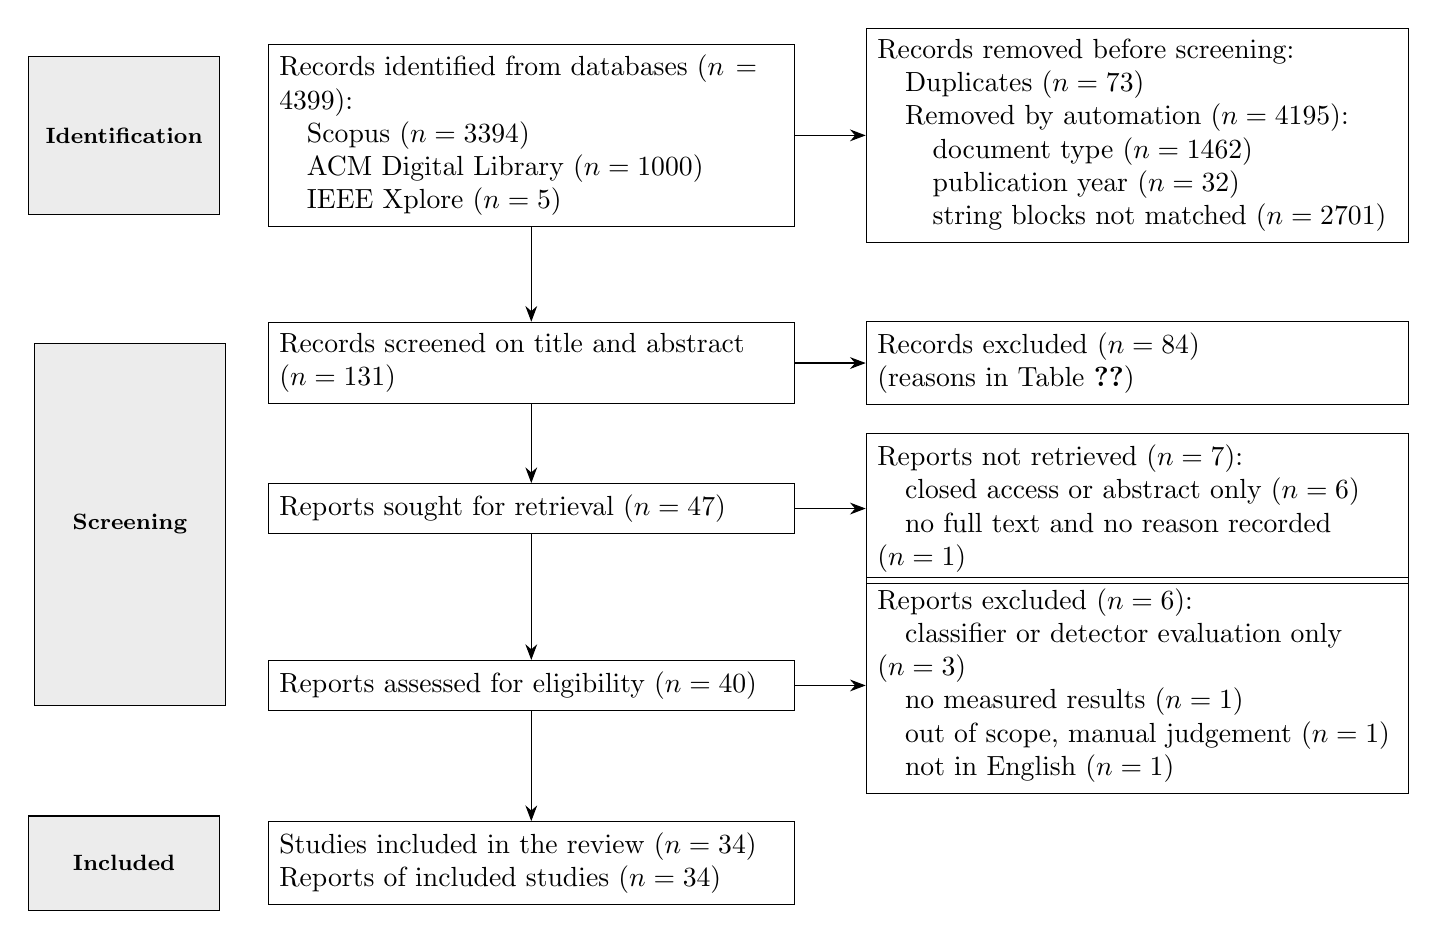
\begin{tikzpicture}[
  node distance=5mm and 9mm,
  box/.style={draw, rectangle, align=left, text width=6.4cm, inner sep=4pt},
  side/.style={draw, rectangle, align=left, text width=6.6cm, inner sep=4pt},
  stage/.style={draw, rectangle, fill=gray!15, minimum height=1.2cm, text width=2.2cm, align=center, font=\footnotesize\bfseries},
  arr/.style={-{Stealth[length=2mm]}}
]
\node[box] (id) {Records identified from databases ($n=\NIdentified$):\\
\quad Scopus ($n=\NScopus$)\\
\quad ACM Digital Library ($n=\NACM$)\\
\quad IEEE Xplore ($n=\NIEEE$)};
\node[side, right=of id] (rm) {Records removed before screening:\\
\quad Duplicates ($n=\NDuplicates$)\\
\quad Removed by automation ($n=\NAuto$):\\
\qquad document type ($n=\NAutoType$)\\
\qquad publication year ($n=\NAutoYear$)\\
\qquad string blocks not matched ($n=\NAutoString$)};

\node[box, below=12mm of id] (scr) {Records screened on title and abstract\\($n=\NScreened$)};
\node[side, right=of scr] (exta) {Records excluded ($n=\NExclTA$)\\(reasons in Table~\ref{tab:tareasons})};

\node[box, below=10mm of scr] (sought) {Reports sought for retrieval ($n=\NSought$)};
\node[side, right=of sought] (nr) {Reports not retrieved ($n=\NNotRetrieved$):\\
\quad closed access or abstract only ($n=\NNotRetClosed$)\\
\quad no full text and no reason recorded ($n=\NNotRetNoRecord$)};

\node[box, below=16mm of sought] (ass) {Reports assessed for eligibility ($n=\NAssessed$)};
\node[side, right=of ass] (exft) {Reports excluded ($n=\NExclFT$):\\
\quad classifier or detector evaluation only ($n=\NFTDetect$)\\
\quad no measured results ($n=1$)\\
\quad out of scope, manual judgement ($n=1$)\\
\quad not in English ($n=1$)};

\node[box, below=14mm of ass] (inc) {Studies included in the review ($n=\NIncluded$)\\Reports of included studies ($n=\NIncluded$)};

\draw[arr] (id) -- (scr);
\draw[arr] (id) -- (rm);
\draw[arr] (scr) -- (sought);
\draw[arr] (scr) -- (exta);
\draw[arr] (sought) -- (ass);
\draw[arr] (sought) -- (nr);
\draw[arr] (ass) -- (inc);
\draw[arr] (ass) -- (exft);

\node[stage, left=6mm of id, minimum height=2.0cm] {Identification};
\node[stage, minimum height=4.6cm] at ($(scr.west)!0.5!(ass.west) + (-17.5mm,0)$) {Screening};
\node[stage, left=6mm of inc] {Included};
\end{tikzpicture}
\caption{PRISMA 2020 flow diagram for new systematic reviews which included searches of databases only. Citation searching was not carried out.}
\label{fig:prisma}
\end{figure*}


Of the \NSought{} reports sought, \NNotRetrieved{} were not retrieved (Table~\ref{tab:notret}). Five were recorded as closed access at retrieval. For a sixth, Wang et al.'s AlertPro, only the publisher's landing page with the abstract and section snippets was obtained, which is not enough to assess the study. For the seventh, no full text is on file and no reason was recorded; this is an unresolved gap in the retrieval record. The remaining \NAssessed{} reports were assessed for eligibility, and \NExclFT{} were excluded (Table~\ref{tab:ftexcl}). Three described response actions but evaluated their models only as classifiers or detectors~\cite{manojkumar2026,bompally2026,reddyavula2026}. One, the shielded incident-response agent of Alauthman et al.~\cite{alauthman2026}, which the project's thematic review had treated as the closest precedent, reports an evaluation plan and ``indicative findings'' shown as arrows, but no measured values. One report was excluded as out of scope on manual judgement, and one because its full text is in French. In all, \NIncluded{} studies, each described in one report, entered the synthesis: \NInclPOne{} from the first priority group and \NInclPTwo{} from the second. Appendix~\ref{app:decisionlog} gives the outcome for every report sought.

\begin{table}[!t]
\centering
\caption{Reports Not Retrieved}
\label{tab:notret}
\footnotesize
\begin{tabularx}{\columnwidth}{@{}lLP{2.6cm}@{}}
\toprule
ID & Report & Reason \\
\midrule
\inputrows{tables/tab_not_retrieved.tex}
\bottomrule
\end{tabularx}
\end{table}

\begin{table*}[!t]
\centering
\caption{Reports Excluded at Full-Text Assessment}
\label{tab:ftexcl}
\footnotesize
\begin{tabularx}{\textwidth}{@{}lP{7.6cm}L@{}}
\toprule
ID & Report & Reason \\
\midrule
\inputrows{tables/tab_ft_exclusions.tex}
\bottomrule
\end{tabularx}
\end{table*}

\subsection{Study Characteristics}

Table~\ref{tab:summary} summarises the \NIncluded{} included studies, and Appendix~\ref{app:characteristics} describes each one. The work is recent: \NYearRecent{} of the \NIncluded{} studies were published in 2025 or 2026, \NYearTwentySix{} of them in 2026, and the earliest in \NYearMin. Most of the evidence comes from security settings. Only \NSetITOPS{} studies concern IT service and cloud operations, and all but one of these address root cause analysis or the remediation of faults in microservice and cloud systems; the exception prioritises incident reports~\cite{peralta2025}. The other \the\numexpr\NIncluded-\NSetITOPS\relax{} studies concern alert triage in security operations centres, incident response on enterprise and military networks, industrial and IoT systems, or digital forensics during incident response.

The environments are mostly constructed. Of the \NIncluded{} studies, \NEnvSim{} built their own simulator and \NEnvBench{} used a public benchmark, chiefly the CAGE-2 and CAGE-4 cyber-defence gyms and the RCAEval root-cause benchmark; \NEnvData{} replayed public datasets, most often intrusion-detection flow records regrouped into decision episodes, and \NEnvEmu{} used emulated testbeds. Only \NEnvOps{} studies used operational data from an organisation~\cite{peralta2025,wang2023hrlhf,ding2023}, and one evaluated on a physical testbed as well as a benchmark~\cite{hammar2026belief}.

\begin{table}[!t]
\centering
\caption{Characteristics of the Included Studies}
\label{tab:summary}
\footnotesize
\begin{tabularx}{\columnwidth}{@{}lLr@{}}
\toprule
Group & Category & Studies \\
\midrule
\inputrows{tables/tab_summary.tex}
\bottomrule
\end{tabularx}
\vspace{2pt}

\raggedright\footnotesize Formulation categories overlap; a study is counted in each that applies, and studies formulated as a fully observed MDP are not listed.
\end{table}

\subsection{Quality of the Included Studies}

The quality of the evidence is uneven (Table~\ref{tab:qualsummary}). Of the \NIncluded{} studies, \NQHigh{} meet at least six of the eight checklist items, and \NQLow{} meet at most two. Hammar et al.~\cite{hammar2026belief} and Sahin and Mert~\cite{sahin2026} meet all eight; Nyberg and Johnson~\cite{nyberg2024} meet seven; Peralta et al.~\cite{peralta2025}, Okafor~\cite{okafor2026}, Rojas Rodriguez et al.~\cite{rojasrodriguez2026}, Ghanem et al.~\cite{ghanem2026}, Hammar and Li~\cite{hammar2025} and Kovtun et al.~\cite{kovtun2026} meet six. The weakly rated studies typically report a single run without variance, do not test the agent on unseen conditions, and describe their environment or hyperparameters too briefly for the work to be repeated. Appendix~\ref{app:quality} gives every rating.

Three weaknesses run across the set. Only \NQFive{} studies report results over several runs with a measure of variance, only \NQSix{} test their agents on conditions not seen in training, and only \NQEight{} give enough detail, with public code or environment, for the work to be repeated. A non-learning baseline is more common, met by \NQThree. The synthesis below therefore gives most weight to the strongly rated studies and treats results from the weakest as indications only.

\begin{table}[!t]
\centering
\caption{Quality Appraisal Summary (\NIncluded{} Studies)}
\label{tab:qualsummary}
\footnotesize
\begin{tabularx}{\columnwidth}{@{}lLrrr@{}}
\toprule
Item & Question & Met & Part & Not \\
\midrule
\inputrows{tables/tab_quality_summary.tex}
\bottomrule
\end{tabularx}
\end{table}

\subsection{Coverage of the Review Questions}

Table~\ref{tab:coverage} counts the studies that contain each element of the review questions, and Fig.~\ref{fig:coverage} shows the same counts against the size of the evidence base. Appendix~\ref{app:coverage} records the elements study by study. The counts are descriptive; no effect sizes were pooled, for the reasons given in Section~\ref{sec:method}.

\begin{table}[!t]
\centering
\caption{Studies Containing Each Element of the Review Questions}
\label{tab:coverage}
\footnotesize
\begin{tabularx}{\columnwidth}{@{}lLr@{}}
\toprule
Group & Element & Studies \\
\midrule
\inputrows{tables/tab_coverage_summary.tex}
\bottomrule
\end{tabularx}
\end{table}

% Coverage of the review-question elements. Counts come from tables/fig_coverage_coords.tex.
\def\CoverageSymbols{{Gathers information},{Response action},{Escalates or defers},{All three decisions},{Hard filter or shield},{Blocked action handled},{Decision quality measured},{Efficiency measured},{Escalation measured},{Compliance measured},{Robustness tested}}
\def\CoverageCoords{(17,{Gathers information}) (22,{Response action}) (7,{Escalates or defers}) (1,{All three decisions}) (5,{Hard filter or shield}) (3,{Blocked action handled}) (31,{Decision quality measured}) (19,{Efficiency measured}) (5,{Escalation measured}) (4,{Compliance measured}) (15,{Robustness tested})}

\begin{figure}[!t]
\centering
\begin{tikzpicture}
\begin{axis}[
  xbar,
  width=0.5\columnwidth,
  height=6.4cm,
  scale only axis,
  xmin=0, xmax=\NIncluded,
  xlabel={Studies (of \NIncluded)},
  symbolic y coords/.expand once=\CoverageSymbols,
  ytick=data,
  y dir=reverse,
  yticklabel style={font=\scriptsize, align=right},
  xticklabel style={font=\scriptsize},
  xlabel style={font=\scriptsize},
  bar width=6pt,
  nodes near coords,
  nodes near coords style={font=\scriptsize},
  enlarge y limits=0.05,
  axis x line*=bottom,
  axis y line*=left,
]
\edef\coverageplot{\noexpand\addplot[fill=gray!60, draw=none] coordinates {\CoverageCoords};}
\coverageplot
\end{axis}
\end{tikzpicture}
\caption{Number of included studies containing each element of the review questions.}
\label{fig:coverage}
\end{figure}


\subsection{Synthesis for SRQ1: Formulation and Representation of Uncertain Evidence}

The answer to SRQ1 is that incident handling is formulated mostly as a fully observed MDP, and that explicit representation of uncertain evidence is the exception. Four themes support this answer.

\emph{1) Explicit belief over a hidden incident state is used by a minority of studies.} Only \NBelief{} studies formulate the problem as a POMDP and act on a belief, a probability distribution over the hidden security state. Hammar et al.\ estimate the belief with a particle filter and compute policies by belief aggregation and rollout~\cite{hammar2026belief}; Hammar and Li go further and hold a belief over the system model itself, updated by Bayesian learning as the incident unfolds~\cite{hammar2025}. Kovtun et al.\ track a belief over a hidden attack regime in a SOC~\cite{kovtun2026}, and Koupaei and Demirkol use a Dempster-Shafer belief for small-enterprise incident response~\cite{koupaei2026}. These are among the more strongly rated studies, so the representation the project needs exists and has been evaluated, although mainly on security benchmarks.

\emph{2) Ambiguity is produced mainly by noisy, missing or overlapping evidence in a simulator, and it is usually fixed at one level.} Koupaei and Demirkol set false-positive and false-negative rates of 12\% and 18\%~\cite{koupaei2026}. Contractor et al.\ lower the detection rate from 95\% to 50\% and add benign users who raise false alerts~\cite{contractor2025}. Sahin and Mert design evidence that is stochastic and overlaps across classes, so that gathering evidence can lower confidence in a true threat or raise it for a benign alert, and add a hardened regime in which threats start at low confidence~\cite{sahin2026}. Wu et al.\ vary fault severity and change the link topology during episodes~\cite{wu2026}, Peralta et al.\ model the vagueness of incident descriptions with fuzzy sets~\cite{peralta2025}, and multi-agent studies give each agent only local observations~\cite{aenugu2026,ravi2025}. Only a few of these studies treat the level of ambiguity as an experimental factor that is varied~\cite{contractor2025,sahin2026,wu2026}.

\emph{3) Many studies treat the incident state as a fully observed feature vector.} In about half the studies the state is a vector of metrics, alert scores or dataset features with no model of what the agent cannot see~\cite{saeed2025,noorulhassan2026,alturkistani2022,bhosale2026,raj2026,nimmathi2026,yuan2026,babar2026,hughes2022,jaber2025,singh2026,ghanem2026,dunsin2025,wang2024mrca,ding2023}. In these studies ambiguity is assumed away rather than modelled, and the agent's decision cannot depend on how certain it is.

\emph{4) No shared environment exists for IT service incident triage.} The security studies share benchmarks: CAGE-2 is used by three studies~\cite{hammar2026belief,hammar2025,nyberg2024} and CAGE-4 or CybORG by two~\cite{castro2025,contractor2025}, and RCAEval serves root cause analysis~\cite{rojasrodriguez2026}. Three studies repurpose intrusion-detection datasets as alert streams or decision episodes~\cite{okafor2026,kovtun2026,alturkistani2022}. Apart from the root-cause studies that use RCAEval or open microservice benchmarks, the IT service studies each build their own fault-injection setup or use one organisation's data~\cite{peralta2025,wang2023hrlhf,ding2023,wu2026,yuan2026}. Results from different IT service studies therefore cannot be compared directly.

\subsection{Synthesis for SRQ2: The Decisions the Agents Make}

The answer to SRQ2 is that gathering information and acting are common decisions, escalation to a person is rare, and no study learns one policy over all three for IT service incidents. Four themes support this answer.

\emph{1) Information gathering is an explicit, costed action in half the studies.} A total of \NInfo{} studies give the agent an action whose purpose is to obtain evidence. In security settings it takes the form of an analyse or investigate action~\cite{hammar2026belief,hammar2025,nyberg2024,castro2025,contractor2025,okafor2026}, queries to logs and threat intelligence~\cite{sahin2026}, a choice of which alerts analysts should investigate within a budget~\cite{tong2020}, a decision to defer and gather context~\cite{kovtun2026}, increased logging~\cite{jaber2025}, or the next step of a forensic examination~\cite{ghanem2026,dunsin2025}. In root cause analysis it is the choice of which part of the system to examine next, whether to stop, or which components to exclude~\cite{rojasrodriguez2026,wang2024mrca,wu2026,ding2023}, and Wang et al.\ let the agent choose which dependencies to ask engineers about~\cite{wang2023hrlhf}.

\emph{2) Where investigation is available, it reduces errors or effort.} Wu et al.\ report 3.2 investigation steps on average against 6.1 for a plain DQN, with higher accuracy~\cite{wu2026}. Kovtun et al.\ find that the option to defer cut false escalations from 7.2\% to 5.0\% and from 9.4\% to 6.6\% on two datasets~\cite{kovtun2026}. Ghanem et al.\ report investigation time cut by up to 68\% against analyst-assisted baselines~\cite{ghanem2026}, and Wang et al.\ reduce the number of questions put to engineers from $O(N^2)$ to $O(1)$~\cite{wang2023hrlhf}. These results support treating investigation as a decision with a cost, as the project does.

\emph{3) Escalation to a person is rarely a learned action.} Only \NEsc{} studies include escalation, deferral or hand-off to a person. Bhosale et al.\ let a DQN choose to allow, monitor or escalate phishing alerts, where escalation opens a ServiceNow incident~\cite{bhosale2026}, and Alturkistani and El-Affendi train a DQN to fix an alert or escalate it to the next tier of SOC operators~\cite{alturkistani2022}. Sahin and Mert's agent can escalate to incident response, and a separate layer defers the most uncertain alerts to an analyst~\cite{sahin2026}; Kovtun et al.'s agent escalates to deep analysis~\cite{kovtun2026}. In the other three the hand-off is fixed by design rather than learned: Okafor leaves containment to analysts in the deployed system~\cite{okafor2026}, Singh routes an action to a human when a deterministic safety check fails~\cite{singh2026}, and Koupaei and Demirkol include notifying a managed security provider as a playbook~\cite{koupaei2026}. Six of the \NEsc{} are in security operations or incident response. The only IT service study among them, Singh's, hands off when a rule check fails; none of the \NSetITOPS{} IT service studies learns when to escalate.

\emph{4) No study learns one policy over investigating, remediating and escalating for IT service incidents.} Only \NAllThree{} study combines an information-gathering action, a response action and escalation: Okafor's offline agents choose to dismiss, investigate or contain SOC alerts, and analyst ownership of containment is a deployment decision, not a learned one~\cite{okafor2026}. Sahin and Mert combine evidence gathering with escalation and closure but have no remediation action~\cite{sahin2026}, and Kovtun et al.\ combine shallow triage, deep analysis and deferral, again without remediation~\cite{kovtun2026}. The three-way decision the project studies is therefore not covered in the evidence base; the nearest work is security alert triage.

\subsection{Synthesis for SRQ3: Enforcement of Operational Constraints}

The answer to SRQ3 is that constraints are most often encoded as reward penalties, that hard rule enforcement is proposed more often than it is measured, and that what replaces a blocked action is almost never reported. Reward penalties are the most common mechanism. A total of \NPenalty{} studies express their operational limits only as penalties in the reward: for destructive self-healing actions~\cite{yuan2026}, for restoring hosts~\cite{nyberg2024,hammar2026belief,hammar2025}, for under-escalation~\cite{bhosale2026}, or for violating an organisation's response policy encoded as a reward profile~\cite{hughes2022}. A further \NNoCon{} state no constraint at all. A penalty discourages a prohibited action but does not prevent it, which is the distinction the project's design depends on~\cite{konighofer2025}. Four themes describe the studies that go further.

\emph{1) Action masking and expected-cost constraints are the common lightweight alternatives.} In \NMask{} studies, actions that are invalid or unsafe in the current state are masked. Contractor et al.\ unmask the disruptive restore action only when a persistent threat is present, and the analyse action only after a detection or a message from another agent~\cite{contractor2025}; root-cause and forensic studies mask expanded nodes or restrict actions to a pool derived from engineers~\cite{wang2024mrca,rojasrodriguez2026,ding2023,ghanem2026,wu2026}. Another \NCostCon{} bound an expected cost or a budget. Kovtun et al.\ constrain both the use of deep analysis and the attack-miss rate, and report that both constraints held in 14 of 15 seeds on one dataset and 13 of 15 on the other~\cite{kovtun2026}; Sahin and Mert certify error budgets on benign escalation and on threats closed automatically, realising rates of 0.0099 and 0.0101 against budgets of 0.01~\cite{sahin2026}.

\emph{2) Hard runtime filters are proposed, but only two studies measure them.} In \NShield{} studies, proposals are checked against rules at run time. Ravi et al.\ check every proposed action against legal, service-level and safety rules and replace a violating action with a safer alternative or a no-op, with a penalty~\cite{ravi2025}. Singh restricts the agent to a feasible action region and adds a deterministic execution guard~\cite{singh2026}. Koupaei and Demirkol restrict the allowable action set by cost and time limits~\cite{koupaei2026}, Elicha and Lopez let expert rules handle known threats before the RL agent sees an alert~\cite{elicha2026}, and Okafor adds a severity floor that prevents medium- and high-severity alerts from being dismissed automatically~\cite{okafor2026}. Only Ravi et al.\ and Singh report how the rules behaved: Ravi et al.'s shield intervened 526 to 623 times per scenario~\cite{ravi2025}, and removing Singh's guard left the mean time to resolution almost unchanged (142~s to 144~s) but cut the governance compliance rate from 99.9\% to 72.3\%~\cite{singh2026}.

\emph{3) What happens to a blocked decision is reported in \NBlocked{} studies.} Ravi et al.\ substitute an alternative or a no-op~\cite{ravi2025}, Singh hands the action to a human~\cite{singh2026}, and Sahin and Mert defer to an analyst any alert that cannot be decided within the error budgets~\cite{sahin2026}. None of the studies lets the agent propose again after a block, which is the project's rule.

\emph{4) Rule enforcement changes behaviour and has a cost.} Singh's guard bought compliance at almost no cost in resolution time~\cite{singh2026}. In Ravi et al.'s study the cost was larger: the shielded agent took 9 to 11 times more false actions and incurred 74--77\% higher cost than an unshielded PPO agent, while detecting far more attacks (recall 0.96--0.99 against 0--0.084)~\cite{ravi2025}. This study is weakly rated, and its text reports that the PPO agent proposed unsafe actions although that agent ran without a shield, so its comparison should be read with caution.

\subsection{Synthesis for SRQ4: Environments, Baselines and Metrics}

The answer to SRQ4 is that the studies measure the quality of the final decision and the time taken, but rarely escalation behaviour or compliance, and that their reporting is often too weak for the results to be compared. Three themes support this answer.

\emph{1) Decision quality and time dominate; escalation and compliance are rarely measured.} Decision quality is measured in \NDQ{} studies, through accuracy, reward, cost, recall or MCC, and \NEff{} studies measure time or investigation effort, most often as mean time to recovery~\cite{singh2026,koupaei2026,nimmathi2026,aenugu2026}. Only \NEscM{} measure escalation behaviour~\cite{peralta2025,sahin2026,nimmathi2026,bhosale2026,kovtun2026} and \NComp{} constraint compliance~\cite{singh2026,sahin2026,kovtun2026,ravi2025}. One study, Kovtun et al., reports measures in all four groups, for SOC alert escalation~\cite{kovtun2026}. Peralta et al.\ report the clearest operational effect on escalation: in a deployment trial, the escalation rate fell from 11.8\% to 9.2\% and manual priority overrides from 15.2\% to 6.2\%, although this was a before--after comparison without a control~\cite{peralta2025}.

\emph{2) A static or rule-based comparison is common but not universal.} In all, \NRuleBase{} studies compare against a non-learning policy: static thresholds, fixed scripts, playbooks, heuristics, a periodic recovery policy, or human examiners~\cite{hammar2026belief,koupaei2026,bhosale2026,wu2026,yuan2026,aenugu2026,ghanem2026}. The others compare only learning methods with each other, compare with values reported by other studies, or have no baseline~\cite{saeed2025,noorulhassan2026,khozam2025,elicha2026,hughes2022,jaber2025,alturkistani2022}. The extracted results contain no case in which a static baseline outperformed the learned policy on a study's main measure. How much this reflects the strength of the learned policies and how much the weakness of the baselines cannot be separated from the reports.

\emph{3) Reporting weaknesses limit the comparisons.} Several studies show how the choice of metric can mislead. Okafor found that value-based offline RL and a Decision Transformer degenerated into trivial detectors whose failure F1 and ROC-AUC concealed and MCC revealed~\cite{okafor2026}. Ravi et al.'s PPO baseline scored 0.98 accuracy with near-zero recall~\cite{ravi2025}. Sahin and Mert report that an earlier version of their simulator leaked the label into the confidence signal, so that any threshold appeared to achieve perfect recall, and recommend checks against this defect~\cite{sahin2026}. Several weaker studies contain internal inconsistencies: two different improvement figures for the same result~\cite{koupaei2026,varsha2025}, a train--test split that is stated but not used~\cite{bhosale2026}, an action in a worked example that is absent from the action set~\cite{jaber2025}, and training and testing on the same stream~\cite{alturkistani2022}.

\subsection{Synthesis for SRQ5: Robustness to Ambiguity and Change}

The answer to SRQ5 is that robustness is tested in under half the studies, mostly for the quality of the final decision, and that no study measures how the mix of investigating, acting and escalating changes as evidence becomes more ambiguous. Three themes support this answer.

\emph{1) Robustness is tested through model error, change, unseen attackers and weaker detection.} A total of \NRobust{} studies test their agents under conditions that differ from training: a misspecified model of the system~\cite{hammar2025}, a non-stationary system~\cite{hammar2026belief}, unseen attacker profiles and network structures~\cite{ravi2025,nyberg2024,castro2025}, a lower detection rate~\cite{contractor2025}, dataset shift~\cite{sahin2026}, terminology drift~\cite{peralta2025}, dynamic topology~\cite{wu2026}, and load near capacity~\cite{aenugu2026,kovtun2026}. Performance generally degrades but does not collapse: Peralta et al.'s accuracy fell from 82.9\% to 79.4\% under drift~\cite{peralta2025}, Aenugu's mean time to recovery rose from 41.2~s to 79.4~s at peak load~\cite{aenugu2026}, and Nyberg and Johnson's graph agents worked on unseen networks without retraining but scored below agents trained on each network~\cite{nyberg2024}.

\emph{2) Methods that maintain a belief or adapt their model degrade least.} Under a misspecified model, Hammar and Li's method incurred a cost of 35.91 against 91.51 or more for every other method, although it was slightly worse than the best methods when the model was correct~\cite{hammar2025}. Hammar et al.'s method adapted its policy to a system change in about 15 to 19 seconds, against more than 30 minutes for PPO, and PPO's results varied about ten times more~\cite{hammar2026belief}. Both studies are strongly rated.

\emph{3) As ambiguity rises, deferral to people rises; how the full decision mix shifts is unmeasured.} Sahin and Mert show that when the scoring model degrades under dataset shift, the share of alerts deferred to analysts rises, to 79--99\% for the most affected classifiers, so that failure becomes visible instead of silent~\cite{sahin2026}. Kovtun et al.\ show that deferring to gather context reduces false escalations~\cite{kovtun2026}, and Contractor et al.\ show that lower detection rates lower returns and that unmasking investigation on a message from another agent recovers part of the loss~\cite{contractor2025}. No study reports the shares of investigating, acting and escalating at increasing levels of ambiguity.

\subsection{Thematic Traceability}

Table~\ref{tab:trace} links each review question to its themes, the studies that support each theme, and the interpretation drawn. It is the basis of the discussion that follows.

\begin{table*}[!t]
\centering
\caption{Thematic Traceability Matrix: Review Question, Theme, Supporting Studies and Interpretation}
\label{tab:trace}
\footnotesize
\begin{tabularx}{\textwidth}{@{}lP{5.2cm}P{4.4cm}L@{}}
\toprule
SRQ & Theme & Supporting studies & Interpretation \\
\midrule
\inputrows{tables/tab_traceability.tex}
\bottomrule
\end{tabularx}
\end{table*}

% ===========================================================================
\section{Discussion}
\label{sec:discussion}
% ===========================================================================

This review set out to find how RL has been applied to IT incident handling, which decisions the agents make, how rules are enforced, and how the agents are evaluated. The \NIncluded{} included studies show that each part of the planned design has been studied somewhere, but not together and seldom for IT service incidents. This section interprets the findings for each review question, returns to the gaps stated in Table~\ref{tab:objectives}, and sets out what the findings imply for the project.

\subsection{Representation of Uncertain Evidence}

The thematic review stated that the environments in the literature model cyberattacks and microservice faults and that none lets the ambiguity of IT service incidents be varied. The systematic search confirms this gap and sharpens it. Belief-based formulations exist and perform well under change~\cite{hammar2026belief,hammar2025}, but all \NBelief{} studies that use them concern security incidents. The IT service studies are almost all root cause analysis on microservice benchmarks or on one company's data, and they treat the system's metrics as fully observed. Three studies vary the level of ambiguity as an experimental factor~\cite{contractor2025,sahin2026,wu2026}; none of them concerns user-reported IT service incidents.

There are two ways to read this. One is that IT service triage does not need a model of hidden state because its evidence is good enough. The studies give no support for this reading, since none tests it. The other is that the field has not yet built an environment in which the question can be asked. Chen et al.'s observation that distinct problems produce similar symptoms~\cite{chen2020} favours the second reading. A simulator in which the overlap between incident causes can be set, as Sahin and Mert do for alert classes~\cite{sahin2026}, would let the question be tested directly.

\subsection{The Three Decisions}

The thematic review found that information gathering and deferral had been studied separately. The included studies agree. Investigation is an explicit action in \NInfo{} studies, and where it is measured it reduces either errors or effort~\cite{wu2026,kovtun2026,ghanem2026,wang2023hrlhf}. Escalation is much rarer, and where it is present it is often fixed by design: a severity floor, a rule-triggered hand-off, or a playbook~\cite{okafor2026,singh2026,koupaei2026}. Only one study combines all three kinds of decision, and its escalation is not learned~\cite{okafor2026}.

The closest work to the project is therefore in security alert triage, not IT service management. Sahin and Mert's system gathers evidence, escalates or closes, and defers the uncertain cases to an analyst under certified error budgets~\cite{sahin2026}. Kovtun et al.'s agent chooses between shallow triage, deep analysis and deferral under a cost constraint~\cite{kovtun2026}. Both are strongly rated, and both treat escalation as a decision with a cost, as Turan et al.\ argue it should be~\cite{turan2026}. Neither recommends a remediation. The project's question is whether one policy can learn to make the choice between all three when the third option is a fix with operational consequences. The evidence does not answer that question; it shows the parts that have worked separately.

\subsection{Enforcement of Operational Rules}

The thematic review found that shields had been demonstrated mainly on control tasks~\cite{alshiekh2018,konighofer2025}, and that the one shielded incident-response agent it identified had not reported how its mechanism behaved~\cite{alauthman2026}. The systematic search confirms that study's status: it reports an evaluation plan and indicative findings, not measurements, and it was excluded on that ground. The \NShield{} included studies with a hard filter show that the idea has reached incident handling, but only two report what the filter did~\cite{ravi2025,singh2026}.

Those two results point in different directions. Singh's guard raised governance compliance from 72.3\% to 99.9\% at almost no cost in resolution time~\cite{singh2026}. Ravi et al.'s shield intervened hundreds of times per scenario and the shielded agent took many more false actions than an unshielded one~\cite{ravi2025}. The difference may lie in how often the agent proposes prohibited actions, which depends on how it was trained. If the agent learns with the shield in place, as Alshiekh et al.\ propose~\cite{alshiekh2018}, it can learn to avoid proposals that will be blocked. Neither study reports the rate of blocked proposals over training, so this explanation cannot be checked from the evidence.

The more important finding for the project is what is missing. Only \NBlocked{} studies say what happens after a block, and none lets the agent propose again. The project's rule, that a blocked agent may make one further proposal before the incident is escalated, has no direct precedent. Its effect on escalation rates and on the time to resolution will have to be measured, not assumed.

\subsection{Environments, Baselines and Metrics}

The thematic review stated that decision quality, investigation cost, escalation and constraint compliance had each been measured but not together. The systematic search finds one exception, Kovtun et al., who measure all four for SOC alert escalation~\cite{kovtun2026}. The rest measure decision quality and time, and few measure escalation or compliance. For an agent whose purpose is to choose between investigating, acting and escalating, decision quality alone is not enough: an agent that escalates every incident makes no wrong fix, and an agent that never escalates may look efficient. Measures of escalation and compliance are needed to see either failure.

The quality appraisal adds a caution about baselines and reporting. A non-learning baseline is common, and the learned policy always beat it in the extracted results, but few studies report variance across runs or test on unseen conditions. Okafor's and Ravi et al.'s results show how a single metric can hide a degenerate policy~\cite{okafor2026,ravi2025}, and Sahin and Mert's account of label leakage in their own simulator shows how a simulator can make a policy look better than it is~\cite{sahin2026}. These are the failure modes the project's evaluation is most exposed to, because it too will train and test in a simulator it builds.

\subsection{Robustness}

The thematic review found that robustness had been tested for decision accuracy and for the validity of shields, but not for the mix of investigating, recommending and escalating. The systematic search confirms this. In \NRobust{} studies the agents are tested under changed conditions, and the methods that maintain a belief or adapt their model degrade least~\cite{hammar2025,hammar2026belief}. Sahin and Mert show the most relevant pattern: as the scoring model degrades, more alerts are deferred to people, so that failure becomes visible~\cite{sahin2026}. No study reports how the shares of the three decisions change as evidence becomes more ambiguous. That curve is what the project's fifth research question asks for.

\subsection{Relevant Excluded Studies}

Two groups of excluded reports bear on the interpretation. The first is the shielded incident-response agent of Alauthman et al.~\cite{alauthman2026}, which the thematic review treated as the closest precedent. Its exclusion leaves no included study that combines a shield with incident response in IT operations and reports measurements. The second is three reports that describe response actions but evaluate their models as classifiers~\cite{manojkumar2026,bompally2026,reddyavula2026}. They show a common pattern in the wider literature: a framework is described as autonomous response, but what is evaluated is detection. A reader who counts such papers as evidence of RL-based response would overestimate how much of that evidence exists.

\subsection{Implications for the Project}

Fig.~\ref{fig:evidence} places the project against the evidence. Each of its four components has a precedent among the included studies, mostly in security settings, and the combination has none. The findings suggest six things for the project's design and evaluation.

\begin{enumerate}
\item The simulator should let the level of ambiguity be set, by controlling how far the symptoms of different causes overlap and how reliable each diagnostic check is, so that robustness can be measured as a function of it~\cite{sahin2026,contractor2025}.
\item The agent should be compared with a learning baseline that keeps a belief, not only with a fully observed one, because belief-based methods were the most robust in the included studies~\cite{hammar2025,hammar2026belief}.
\item Escalation should be a learned action with a cost, and its rate should be reported alongside decision quality, so that an agent which escalates everything cannot appear safe~\cite{kovtun2026,turan2026}.
\item The rule mechanism should log every block, the re-proposal that follows, and whether the incident was then escalated, because no included study reports this sequence.
\item Results should be reported over several seeds with variance, with more than one decision-quality metric, and with checks for label leakage in the simulator~\cite{okafor2026,sahin2026}.
\item The static, rule-based baseline should be as strong as a competent support team would use, because a weak baseline makes any learned policy look good.
\end{enumerate}

\begin{figure}[!t]
\centering
\footnotesize
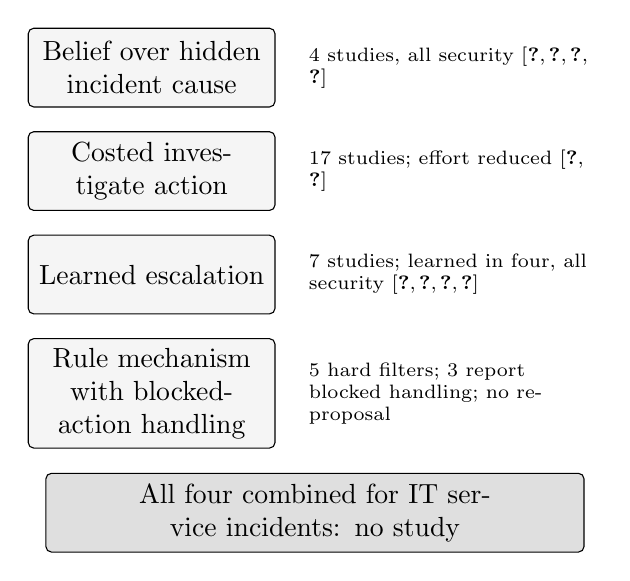
\begin{tikzpicture}[
  comp/.style={draw, rectangle, rounded corners=2pt, align=center, text width=2.9cm, minimum height=1.0cm, fill=gray!8},
  ev/.style={align=left, text width=3.6cm, font=\scriptsize},
  node distance=3mm
]
\node[comp] (c1) {Belief over hidden incident cause};
\node[ev, right=of c1] (e1) {\NBelief{} studies, all security~\cite{hammar2026belief,hammar2025,kovtun2026,koupaei2026}};
\node[comp, below=of c1] (c2) {Costed investigate action};
\node[ev, right=of c2] (e2) {\NInfo{} studies; effort reduced~\cite{wu2026,kovtun2026}};
\node[comp, below=of c2] (c3) {Learned escalation};
\node[ev, right=of c3] (e3) {\NEsc{} studies; learned in four, all security~\cite{bhosale2026,alturkistani2022,sahin2026,kovtun2026}};
\node[comp, below=of c3] (c4) {Rule mechanism with blocked-action handling};
\node[ev, right=of c4] (e4) {\NShield{} hard filters; \NBlocked{} report blocked handling; no re-proposal};
\node[comp, fill=gray!25, text width=6.6cm, anchor=north] (all) at ($(c4.south west)!0.5!(e4.south east)+(0,-4mm)$) {All four combined for IT service incidents: no study};
\end{tikzpicture}
\caption{The components of the planned agent and the included evidence for each.}
\label{fig:evidence}
\end{figure}

% ===========================================================================
\section{Limitations}
\label{sec:limitations}
% ===========================================================================

The limitations of this review lie in the evidence it found and in the way it was conducted.

\subsection{Limitations of the Evidence}

Most of the evidence comes from simulation. Of the \NIncluded{} studies, \NEnvSim{} built their own simulator, and only \NEnvOps{} used an organisation's operational data. Results from a simulator show what a policy can learn from the dynamics its authors chose, not how it will behave on real incidents. The evidence also leans towards security. Of the \NIncluded{} studies, \the\numexpr\NIncluded-\NSetITOPS\relax{} concern security operations, incident response, industrial systems or forensics, and most of the \NSetITOPS{} IT service studies concern root cause analysis rather than triage. Findings carried over from security alert triage to IT service incidents assume that the two decision problems are alike, which the studies do not test.

The quality of the evidence is uneven. Of the included studies, \NQLow{} meet at most two of the eight checklist items, only \NQFive{} report variance over repeated runs, and only \NQEight{} give enough detail to repeat the work. Several studies contain internal inconsistencies (Section~\ref{sec:results}). The checklist itself was written for this review and has not been validated, so the ratings indicate reporting quality and should not be read as a measure of risk of bias. The studies differ too much in task, environment and metric for their results to be pooled, so the synthesis is narrative and the counts are descriptive.

\subsection{Limitations of the Review Process}

The search may have missed relevant studies. Only three databases were searched, and Web of Science and arXiv were not among them. The IEEE Xplore search was limited to open-access records and returned \NIEEE, so IEEE studies behind a paywall that Scopus does not index are missing. The ACM Digital Library export reached its limit of \NACM{} records, so records beyond that limit were not seen; most of the exported ACM records were proceedings volumes, which suggests that the all-fields search was too broad for that library. The year terms in the Scopus and ACM strings do not restrict publication year, and the year filter was applied afterwards by the script. Citation searching was planned but not carried out, and at least one known relevant study was therefore not found~\cite{ren2025}.

Automated filtering removed \NAuto{} records by applying the string blocks to titles, abstracts and keywords. A relevant study that uses none of the method terms in these fields would have been removed without being read. Records without an abstract were judged on their titles alone.

Seven reports could not be assessed. Five were closed access, only the landing page of a sixth was obtained, and for the seventh no full text is on file and no reason was recorded. One report was excluded because its full text is in French. The review cannot say whether these eight reports would have changed its findings; at least three of the unretrieved reports concern SOC alert prioritisation, which is close to the review's focus.

Screening and extraction were not duplicated. The title and abstract decisions, the full-text assessments of the reports on file, the extraction and the quality ratings were made with an AI assistant, and two full-text decisions were made manually. The decision log, the extraction file and the quality ratings are provided so that every decision can be checked. Finally, the review was written to prepare for a particular study, and the themes were coded against that study's design. Section~\ref{sec:screening} and Appendix~\ref{app:decisionlog} state the decisions that required interpretation so that a reader can judge whether this framing affected them.

% ===========================================================================
\section{Future Research}
\label{sec:future}
% ===========================================================================

The gaps identified by this review suggest four directions for research, and two for the review itself.

The first is an environment for IT service incident triage in which the ambiguity of the evidence can be controlled. No such environment was found. It should let a researcher set how far the symptoms of different causes overlap and how reliable each diagnostic check is, and it should be released with its code so that results can be compared across studies, as the CAGE gyms allow for cyber defence.

The second is a single policy that learns to investigate, recommend a fix or escalate, evaluated against both a static policy and learning baselines with and without a belief. The security studies of Sahin and Mert~\cite{sahin2026} and Kovtun et al.~\cite{kovtun2026} show that parts of this design work for alerts; whether they work together when one option changes the system is an open question.

The third is the behaviour of rule enforcement when the agent can also investigate or escalate. Studies should report how often proposals are blocked during training and evaluation, what replaces a blocked proposal, and how blocking changes the rates of investigation and escalation. Only \NBlocked{} included studies report any part of this.

The fourth is evaluation practice. Studies should report decision quality, investigation cost, escalation behaviour and compliance together; results over several seeds with variance; and performance as a function of ambiguity, including the shares of the three decisions at each level. Checks for label leakage in simulators, of the kind Sahin and Mert describe~\cite{sahin2026}, should be routine.

For the review itself, the citation searching that was planned should be carried out, and the IEEE Xplore and ACM Digital Library searches should be repeated, the first without the open-access limit and the second restricted to titles, abstracts and keywords. The seven reports that could not be retrieved should be obtained and assessed.

% ===========================================================================
\section{Conclusion}
\label{sec:conclusion}
% ===========================================================================

This review searched three databases for studies that apply RL or sequential decision-making to IT incident handling, screened \NScreened{} records, and included \NIncluded{} studies. Its findings answer the five review questions. Most studies formulate incident handling as a fully observed MDP, and only \NBelief{} keep an explicit belief over the hidden state. Information gathering is a common action, but escalation to a person is rare and often fixed by design, and only one study combines gathering, acting and escalating. Rule enforcement is usually a reward penalty; hard filters appear in \NShield{} studies, and only \NBlocked{} say what happens to a blocked decision. Decision quality is measured almost everywhere, while escalation and compliance are measured in few studies, and robustness is tested for the final decision but not for the mix of decisions.

The parts of an agent that investigates, acts or escalates under explicit rules have each been studied, mostly for security incidents, but no included study combines them for IT service incidents. The evidence is recent, largely simulated and uneven in quality. Within those limits, the review supports the project's plan to study such an agent, and it indicates what the evaluation must include: controlled ambiguity, learned escalation with a cost, a record of every blocked proposal, and measures of escalation and compliance reported alongside decision quality.


\section*{Declaration of AI Assistance}
Claude (Anthropic) supported the development of search strings and eligibility criteria, data-processing scripts, screening, data extraction, and quality appraisal. The database searches and full-text retrieval, the review’s direction and framing, and the full-text decisions for two reports were completed independently of the assistant.


\bibliographystyle{IEEEtran}
\bibliography{references}

\onecolumn
\appendices
% ===========================================================================
\section{Decision Log for Reports Sought}
\label{app:decisionlog}
% ===========================================================================

The table lists every report sought for retrieval, with its priority group from title and abstract screening (1 or 2) and its outcome. The decisions for all \NScreened{} screened records are in \texttt{audit/exclusion\_traceability.csv} and in the screening record.

\begin{center}\refstepcounter{table}\label{tab:decisionlog}\footnotesize
\MakeUppercase{\tablename}~\thetable\\[2pt]\textsc{Outcome of Every Report Sought for Retrieval}\end{center}
\vspace{-6pt}
{\footnotesize
\begin{longtable}{@{}p{0.6cm}p{9.6cm}p{0.7cm}p{0.6cm}p{4.2cm}@{}}
\toprule
ID & Report & Year & Prio. & Outcome \\
\midrule
\endfirsthead
\toprule
ID & Report & Year & Prio. & Outcome \\
\midrule
\endhead
\bottomrule
\endfoot
\inputrows{tables/tab_decisionlog_long.tex}
\end{longtable}
}

% ===========================================================================
\section{Characteristics of the Included Studies}
\label{app:characteristics}
% ===========================================================================

\begin{center}\refstepcounter{table}\label{tab:characteristics}\footnotesize
\MakeUppercase{\tablename}~\thetable\\[2pt]\textsc{Task, Formulation, Environment and Main Result of Each Included Study}\end{center}
\vspace{-6pt}
{\footnotesize
\begin{longtable}{@{}p{2.3cm}p{0.7cm}p{2.8cm}p{3.3cm}p{3.0cm}p{3.9cm}@{}}
\toprule
Study & Year & Task & Formulation; method & Environment or data & Main reported result \\
\midrule
\endfirsthead
\toprule
Study & Year & Task & Formulation; method & Environment or data & Main reported result \\
\midrule
\endhead
\bottomrule
\endfoot
\inputrows{tables/tab_characteristics_long.tex}
\end{longtable}
}

% ===========================================================================
\section{Decisions, Constraints and Robustness in Each Included Study}
\label{app:coverage}
% ===========================================================================

A dash means the element is absent or not reported.

\begin{center}\refstepcounter{table}\label{tab:coveragelong}\footnotesize
\MakeUppercase{\tablename}~\thetable\\[2pt]\textsc{Coding of the Review-Question Elements for Each Included Study}\end{center}
\vspace{-6pt}
{\footnotesize
\begin{longtable}{@{}p{2.3cm}p{2.9cm}p{2.9cm}p{2.4cm}p{2.9cm}p{2.6cm}@{}}
\toprule
Study & Information gathering & Response action or disposition & Escalation & Constraint (and blocked-action handling) & Robustness test \\
\midrule
\endfirsthead
\toprule
Study & Information gathering & Response action or disposition & Escalation & Constraint (and blocked-action handling) & Robustness test \\
\midrule
\endhead
\bottomrule
\endfoot
\inputrows{tables/tab_coverage_long.tex}
\end{longtable}
}

% ===========================================================================
\section{Quality Appraisal of Each Included Study}
\label{app:quality}
% ===========================================================================

Items Q1--Q8 are defined in Table~\ref{tab:checklist}. ``Items met'' counts only the items rated Yes.

\begin{center}\refstepcounter{table}\label{tab:quality}\footnotesize
\MakeUppercase{\tablename}~\thetable\\[2pt]\textsc{Quality Ratings of the Included Studies}\end{center}
\vspace{-6pt}
{\footnotesize
\begin{longtable}{@{}p{3.6cm}*{8}{>{\centering\arraybackslash}p{0.9cm}}>{\centering\arraybackslash}p{1.2cm}@{}}
\toprule
Study & Q1 & Q2 & Q3 & Q4 & Q5 & Q6 & Q7 & Q8 & Items met \\
\midrule
\endfirsthead
\toprule
Study & Q1 & Q2 & Q3 & Q4 & Q5 & Q6 & Q7 & Q8 & Items met \\
\midrule
\endhead
\bottomrule
\endfoot
\inputrows{tables/tab_quality_long.tex}
\end{longtable}
}


\end{document}
